%!TEX program = lualatex
%!TEX encoding = UTF-8 Unicode  
%!TEX root = chapter02.tex  
\documentclass[main.tex]{subfiles} 
\begin{document} 
%----------------------------------------------------------------------------------------
%	CHAPTER 1
%----------------------------------------------------------------------------------------
\cleardoublepage 
\loadgeometry{marginlayout}  
\pagestyle{scrheadings} % Print headers again  
\KOMAoptions{
	headwidth=textwithmarginpar,
	headsepline=true,
	headsepline= 0.5pt,
	footwidth=textwithmarginpar,
}   
\onehalfspacing 
\setcounter{chapter}{1}
\chapter{Fractions et puissances}

\section{Arithmétique sur les nombres rationnels}
Entrainement \url{http://mathsmentales.net/}
\begin{itemize}
	\item inverse de décimaux classiques, d'entiers, de fractions avec notation puissance \url{http://bref.jeduque.net/2nwzhd}
	\item  multiplication de fractions \url{http://bref.jeduque.net/us89im}
	\item division de fractions \url{http://bref.jeduque.net/0sdpuf}
	\item  addition/soustraction de fractions, niveau 5\ieme \url{http://bref.jeduque.net/log0ei}
	\item addition/soustration et simplification de fractions, niveau 4\ieme  \url{http://bref.jeduque.net/qxlwy1} 
\end{itemize} 
  
%----------------------------------------------------------------------------------------
%	EXERCICES
%----------------------------------------------------------------------------------------

\newpage 
\loadgeometry{widelayout}  
\pagestyle{scrheadings} % Print headers again  
\KOMAoptions{
	headwidth=textwithmarginpar,
	headsepline=true,
	headsepline= 0.5pt,
	footwidth=textwithmarginpar,
} 
\onehalfspacing
\subsection{Exercices fractions et nombres rationnels}



\begin{exercise}[\cancel{\faCalculator}] Ecrire les inverses demandés sous la forme d'une fraction irréductible.
	
	\begin{multicols}{3}
		\begin{enumerate}[label={\alph*)\rule{0pt}{1.8em}},leftmargin=*]
			\item $48^{-1}=$ 
			\item $46^{-1}=$
			\item $44^{-1}$
			\item inverse de $1=$
			\item inverse de $10=$
			\item inverse de $24=$
			\item $\numprint{13}^{-1}=$ 
			\item inverse de $\frac{19}{10}=$
			\item $\left(\frac{-10}{-2}\right)^{-1}=$ 
			\item $\left(\frac{2}{14}\right)^{-1}=$ 
			\item $\left(\frac{14}{4}\right)^{-1}=$ 
			\item $\left(\frac{1}{15}\right)^{-1}=$ 
			\item $\left(\frac{1}{20}\right)^{-1}=$ 
		\end{enumerate}
	\end{multicols}
\end{exercise}
\begin{exercise}\hfill 
	\begin{enumerate}[label={\arabic*)\rule{0pt}{1.6em}},leftmargin=*]
		\item  Compléter pour convertir les décimaux suivants en fractions irréductibles.
	\begin{multicols}{2}
	\begin{enumerate}[label={\alph*)\rule{0pt}{1.6em}},leftmargin=*]
		\item $\numprint{2.25}=\frac{\ldots}{100}=\frac{4\times \ldots}{4\times \ldots }=\frac{\ldots}{\ldots}$
		\item $\numprint{1.6}=\frac{\ldots}{10}=\frac{2\times \ldots}{2\times \ldots }=\frac{\ldots}{\ldots}$ 
		\item $\numprint{0.125}=\frac{\ldots}{1000}=\frac{125\times \ldots}{125\times \ldots }=\frac{\ldots}{\ldots}$ 
		\item $\numprint{0.05}=\frac{\ldots}{100}=\frac{125\times \ldots}{125\times \ldots }=\frac{\ldots}{\ldots}$  
	\end{enumerate}
\end{multicols}
	\item Sans aucun calcul supplémentaire, en déduire les inverses suivants : 
		\begin{multicols}{4}
		\begin{enumerate}[label={\alph*)\rule{0pt}{1.8em}},leftmargin=*]
			\item $\numprint{2.25}^{-1}=$
			\item $\frac{1}{\numprint{1.6}}=$
			\item $\numprint{0.125}^{-1}=$
			\item $\frac{1}{\numprint{0.05}}=$
		\end{enumerate}
	\end{multicols}
\end{enumerate}
\end{exercise}
\begin{exercise}[\cancel{\faCalculator}] Donner l'écriture décimale de l'inverse de décimaux classiques suivants :
	
	\begin{multicols}{4}
		\begin{enumerate}[label={\alph*)\rule{0pt}{1.6em}},leftmargin=*]
			\item $\frac{1}{4}=$
			\item $\frac{1}{40}=$
			\item $\frac{1}{20}=$ 
			\item $\frac{1}{\numprint{0.2}}=$ 
			\item $5^{-1}=$
			\item $50^{-1}=$
			\item $1000^{-1}=$  
			\item $\frac{1}{\numprint{0.01}}=$ 
		\end{enumerate}
	\end{multicols}
\end{exercise}
\begin{example}[\cancel{\faCalculator}, je fais] Donner l'écriture en fraction irréductible des produits et quotients suivants :

\noindent\hfill\parbox{0.23\linewidth}{	
	$\begin{WithArrows}
		A& =\frac{10}{9}\times \frac{-7}{2}\rule{0pt}{1.8em}  \\
		 &=\frac{-10 \times 7}{3\times 3 \times 2}\rule{0pt}{1.8em}  \\
		 & = \frac{-5\times 2 \times 7}{3\times 3 \times 2}\rule{0pt}{1.8em}  \\ 
		 & = \rule{0pt}{1.8em}  \\ 
		 & = \rule{0pt}{1.8em} 
	\end{WithArrows}$ 	
} \hfill\parbox{0.23\linewidth}{	
	$\begin{WithArrows}
		B& =\frac{11}{7}\times \frac{9}{10}\rule{0pt}{1.8em} \\
		&= \rule{0pt}{1.8em} \\
		& = \rule{0pt}{1.8em}  \\ 
		& = \rule{0pt}{1.8em}  \\ 
		& = \rule{0pt}{1.8em} 
	\end{WithArrows}$ 	
}  \hfill\parbox{0.23\linewidth}{	
	$\begin{WithArrows}
		C& =\dfrac{\dfrac{11}{4}}{\dfrac{6}{8}}\\
		&= \rule{0pt}{1.8em} \\
		& = \rule{0pt}{1.8em}  \\ 
		& = \rule{0pt}{1.8em}  \\ 
		& = \rule{0pt}{1.8em} 
	\end{WithArrows}$
}  \hfill\parbox{0.23\linewidth}{	
	$\begin{WithArrows}
		D& =\frac{-11}{9}\divisionsymbol\frac{5}{18} \rule{0pt}{1.8em} \\
		&= \rule{0pt}{1.8em} \\
		& = \rule{0pt}{1.8em}  \\ 
		& = \rule{0pt}{1.8em}   \\ 
		& = \rule{0pt}{1.8em} 
	\end{WithArrows}$
}  
\end{example}
\begin{exercise}[\cancel{\faCalculator}] Mêmes consignes
	
	\begin{multicols}{4}
		\begin{enumerate}[label={$\Alph*=$\rule{0pt}{1.6em}},leftmargin=*]
			\item $\frac{5}{6}\times \frac{8}{-5}$ 
			\item $\frac{8}{5}\times \frac{3}{10}$ 
			\item $\frac{-8}{7}\times \frac{5}{5}$ 
			\item $\frac{-11}{7}\times \frac{-9}{-10}$ 
			\item $\left(\frac{5}{6} \right)^2$   
			\item $ \frac{2}{3}\divisionsymbol \frac{7}{4}  $   
			\item $\frac{5}{-8}\divisionsymbol \frac{13}{9}$ 
			\item $ \frac{-13}{9} \divisionsymbol \frac{-5}{8} $ 
		\end{enumerate}
	\end{multicols}
\end{exercise}
\begin{example}[\cancel{\faCalculator}, je fais] Donner l'écriture en fraction irréductible des produits et quotients suivants :
	
	\noindent\hfill\parbox{0.22\linewidth}{	
		$\begin{WithArrows}
			A& =2+\frac{7}{-30}\rule{0pt}{1.8em}  \\
			&= \rule{0pt}{1.8em}  \\
			& =  \rule{0pt}{1.8em}  \\ 
			& = \rule{0pt}{1.8em}  
		\end{WithArrows}$ 	
	} \hfill\parbox{0.22\linewidth}{	
		$\begin{WithArrows}
			B& =2\times \frac{7}{-30}\rule{0pt}{1.8em} \\
			&= \rule{0pt}{1.8em} \\
			& = \rule{0pt}{1.8em}  \\ 
			& = \rule{0pt}{1.8em}   
		\end{WithArrows}$ 	
	}  \hfill\parbox{0.22\linewidth}{	
		$\begin{WithArrows}
			C& =\frac{-7}{5} -\frac{17}{20}\rule{0pt}{1.8em} \\
			&= \rule{0pt}{1.8em} \\
			& = \rule{0pt}{1.8em}  \\ 
			& = \rule{0pt}{1.8em}   
		\end{WithArrows}$
	}  \hfill\parbox{0.22\linewidth}{	
		$\begin{WithArrows}
			D& =\frac{2}{6}-\frac{7}{18}\rule{0pt}{1.8em} \\
			&= \rule{0pt}{1.8em} \\
			& = \rule{0pt}{1.8em}  \\ 
			& = \rule{0pt}{1.8em}    
		\end{WithArrows}$
	}  
\end{example}

\begin{exercise}[\cancel{\faCalculator}] Écrire sous forme d'une fraction irréductible les expressions suivantes. Détailler les étapes.
	
	\begin{multicols}{4}
		\begin{enumerate}[label={$\Alph*=$\rule{0pt}{1.8em}},leftmargin=*] 
			\item $ 3+ \frac{-7}{5}$
			\item $ 3\times \frac{-7}{5}$
			\item $  \frac{3}{25} - 2$ 
			\item $\frac{8}{11}\divisionsymbol 5$ 
			\item $ -\frac{2}{7}+\frac{5}{21}$
			\item $ 3+ \frac{-7}{5} \times \frac{17}{20}$
			\item $  \dfrac{9}{8} +\dfrac{15}{24}$
%			\item $  \frac{7}{6}+\frac{7}{18}$
			\item $ \frac{7}{12}-\frac{1}{8}$ 
			\item $\dfrac{1}{8}-\dfrac{7}{12}$ 
			\item $ -\frac{4}{15}  +\frac{7}{-30} $ 
			\item $ \frac{3}{20}+\frac{4}{25}$ 
			\item 	$  1- \frac{4}{15}\times\frac{7}{6}$   
		\end{enumerate}
	\end{multicols}
\end{exercise} 

\begin{exercise} 
	Une population de bactéries est multipliée par $5$ à chaque heure quand les conditions sont bonnes.
	\begin{enumerate}[label=\arabic*),leftmargin=*]
		\item Par quel nombre est multipliée la population en  2 h ? en 6 h? en $x$ heures ? en $2x$ heures ?
		\item On décide d'éliminer les $90\%$ des bactéries toutes les deux heures.  
		
		 Par quel nombre est multipliée la population globale après 2 h ? 4 h ? après $2x$ heures ? 
	\end{enumerate}  
\end{exercise}

%----------------------------------------------------------------------------------------
% 
%----------------------------------------------------------------------------------------

\newpage 
\loadgeometry{marginlayout}  
\pagestyle{scrheadings} % Print headers again  
\KOMAoptions{
	headwidth=textwithmarginpar,
	headsepline=true,
	headsepline= 0.5pt,
	footwidth=textwithmarginpar,
} 
\onehalfspacing  

\section{Notation puissances}
\begin{marginfigure}
\begin{tikzpicture}
	\node[circle , draw , minimum size=3cm] (output) [thick, font=\fontsize{40}{0}\selectfont, thick] {$2^4$};
	\node (puissance) [thick, rectangle, draw, font=\fontsize{10}{0}\selectfont, below right=0.3cm and 1.3cm of output] {puissance};
	\node (exposant) [thick, rectangle, draw, font=\fontsize{10}{0}\selectfont, above right=0.1cm and 0.7cm of output] {exposant};
	\node (base) [thick, rectangle, draw, font=\fontsize{10}{0}\selectfont, below left=0.25cm and 0.25cm of output] {base};
	\draw[line width=1mm, ->] (puissance) -- (output);
	\draw[line width=1mm, ->] (base) --++ (1.2cm,1.2cm);
	\draw[line width=1mm, ->] (exposant) --++ (-1.8cm,-1.0cm);
\end{tikzpicture}
\caption{\og $2$ à la puissance $4$ \fg{}\\
	\og $2$ élevée à la puissance $4$ \fg{}\\ 
	\og $2$ puissance $4$ \fg{}\\
	\og $2$ exposant $4$ \fg{} }
\end{marginfigure}
\begin{tBox}[frametitle={Les puissances de $a$}] 
	Pour tout nombre positif ou négatif $a$ : 
	
	$\begin{aligned}
		a^0 & = 1\\
		a^1 & =  a\\
		a^2 & =  a\times a \\
		a^3 & = a\times a\times a\\
		a^4 & = a\times a\times a\times a\\
		a^5 & =  a\times a\times a\times a\times a %\\
		%		a^6 & =  a\times a\times a\times a\times a\times a\\
	\end{aligned}$  
\end{tBox}  
\begin{tBox} Pour tout nombre $a$ non nul, 	$a^{-1}$ désigne l' \og inverse de $a$\fg{}.
	\[
	a^{-1}= \frac{1}{a} \qquad \frac{1}{a^{-1}}=a
	\] 
\end{tBox}
\begin{tBox} Pour tout entier $n$ négatif.
	
	
	$a^{-n}$ désigne l' \og inverse de $a^n$\fg{} ou encore  \og (inverse de $a$) à la puissance $n$ \fg{}.
	\[
	a^{-n}= \frac{1}{a^n} = \left(\frac{1}{a}\right)^n \qquad \frac{1}{a^{-n}}=a^n
	\] 
\end{tBox}

\begin{example}
	Pour tout nombre non nul $a$ : 
	
	$\begin{aligned}
		%	a^{-1} & = \frac{1}{a^1}\\
		a^{-2} & = \frac{1}{a^2} =\frac{1}{a\times a}=\frac{1}{a}\times \frac{1}{a} = \left(\frac{1}{a}\right)^2 \\ 
		a^{-3} & =\frac{1}{a^3}=\frac{1}{a\times a \times a} =\frac{1}{a}\times \frac{1}{a}\times \frac{1}{a} = \left(\frac{1}{a}\right)^3\\ 
		a^{-4} & =\frac{1}{a^4}   = \left(\frac{1}{a}\right)^4 
	\end{aligned}$ \\
 $\begin{aligned}
		5^{-1}& =\qquad \qquad  &
		5^{-2}& = \\
		\left(\frac{1}{5}\right)^{-1}&= &
		\left(\frac{1}{5}\right)^{-2}&= \\  
		\left(\frac{-1}{5}\right)^{-2}&= &
		\left(\frac{2}{3}\right)^{-1}&= \\
		\left(\frac{-2}{3}\right)^{-1}&= &
		\left(\frac{-2}{3}\right)^{-4}&= \\
		%		a^{-5} & =\frac{1}{a^5}= \left(\frac{1}{a}\right)^5% \\
		%		a^{-6} & = 1\divisionsymbol a^6=\frac{1}{a^6}= \left(\frac{1}{a}\right)^6\\
	\end{aligned}$ 
\end{example} 


%----------------------------------------------------------------------------------------
% 
%----------------------------------------------------------------------------------------

\newpage 
\loadgeometry{marginlayout}  
\pagestyle{scrheadings} % Print headers again  
\KOMAoptions{
	headwidth=textwithmarginpar,
	headsepline=true,
	headsepline= 0.5pt,
	footwidth=textwithmarginpar,
} 
\onehalfspacing  



\section{Opérations sur les puissances}

\begin{theorem}[Multiplication de puissances de même base]
	Pour tous entiers $m, n$ (positifs ou négatifs), et tous nombres $a, b$ non nuls : 
	$$
	a^m\times a^n   =a^{m+n}  \qquad 
	\frac{a^m}{a^n}   = a^{m-n} =\frac{1}{a^{n-m}}  
	$$
	\og je multiplie des puissances, les bases sont les mêmes, j'ajoute les exposants \fg{} 
\end{theorem}
\begin{example}\hfill 
	\begin{align*}
		a^2 \times a^3 &= a\times a \times a \times a \times a & 5a^2 \times 7a^3& = 5aa \times 7 aaa \\
		& =a^5 & & = 5\times 7\times aaaaa\\
		&&& =35 a^5 \\
		a^2\times a^{-3}& = \frac{a^2}{a^3}  & a^{-2}\times a^3 & = \frac{a^3}{a^2} \\
		& = \frac{aa}{aaa} && = \frac{aaa}{aa} \\
		& = \frac{1}{a}=a^{-1} && =a
	\end{align*}
\end{example} 
\begin{theorem}[Puissance d'une puissance]
	Pour tous entiers $m, n$ (positifs ou négatifs), et tous nombres $a, b$ non nuls : 
	$$
	(a^n )^m  = a^{nm} 
	$$ 
\end{theorem}

\begin{theorem}[Multiplication de puissances de même exposant]
	Pour tous entiers $m, n$ (positifs ou négatifs), et tous nombres $a, b$ non nuls :
	$$
	(ab)^n = a^n b^n \qquad  \left(\frac{a}{b}\right)^n  = \frac{a^n}{b^n}
	$$
	\og la puissance d'un produit est le produit des puissances \fg{} 
\end{theorem}
\begin{remark}
	Retenir surtout le cas particulier $n=2$ :
	$$
	(ab)^2 = a^2 b^2 \qquad  \left(\frac{a}{b}\right)^2  = \frac{a^2}{b^2}
	$$
\end{remark}


%----------------------------------------------------------------------------------------
%	EXERCICES
%----------------------------------------------------------------------------------------

\newpage 
\loadgeometry{widelayout}  
\pagestyle{scrheadings} % Print headers again  
\KOMAoptions{
	headwidth=textwithmarginpar,
	headsepline=true,
	headsepline= 0.5pt,
	footwidth=textwithmarginpar,
} 
\onehalfspacing
\subsection{Exercices puissances de base quelconque}
\begin{example}[\cancel{\faCalculator}, je fais] Donner l'écriture entière les expressions suivantes.
	
	\noindent\hfill\parbox{0.22\linewidth}{	
		$\begin{WithArrows}
			A& =(-4)^2\rule{0pt}{1.8em}  \\
			&= \rule{0pt}{1.8em}  \\
			& =  \rule{0pt}{1.8em}  
		\end{WithArrows}$ 	
	} \hfill\parbox{0.22\linewidth}{	
		$\begin{WithArrows}
			B& =-4^2\rule{0pt}{1.8em} \\
			&= \rule{0pt}{1.8em} \\
			& = \rule{0pt}{1.8em}    
		\end{WithArrows}$ 	
	}  \hfill\parbox{0.22\linewidth}{	
		$\begin{WithArrows}
			C& =(-4)^3\frac{-7}{5} -\frac{17}{20}\rule{0pt}{1.8em} \\
			&= \rule{0pt}{1.8em} \\
			& = \rule{0pt}{1.8em}   
		\end{WithArrows}$
	}  \hfill\parbox{0.22\linewidth}{	
		$\begin{WithArrows}
			D& =-4^3\rule{0pt}{1.8em} \\
			&= \rule{0pt}{1.8em} \\
			& = \rule{0pt}{1.8em}    
		\end{WithArrows}$
	}  
\end{example}

\begin{exercise}[\cancel{\faCalculator}, à vous] Donner l'écriture entière les expressions suivantes.
	
	\begin{multicols}{4}
	\begin{enumerate}[label={$\Alph*=$\rule{0pt}{1.6em}},leftmargin=*] 
		\item $-6^2$
		\item $(-6)^2$
		\item $5^3$
		\item $-5^3$
		\item $(-5)^3$
		\item $-1^2$
		\item $(-1)^2$
		\item $-(-1)^2$
		\item $-2^3$
		\item $-(3)^4$
		\item $-(-4)^2$
		\item $(-8)^2$
\end{enumerate}
\end{multicols}
\end{exercise}
\begin{example}[\cancel{\faCalculator}, je fais] Donner l'écriture simplifiée des expressions suivantes sous forme d'entiers ou de fractions irréductibles
	
	\noindent\hfill\parbox{0.19\linewidth}{	
		$\begin{WithArrows}
			A& =4^0\rule{0pt}{1.8em}  \\
			&= \rule{0pt}{1.8em}  \\
			& =  \rule{0pt}{1.8em}  
		\end{WithArrows}$ 	
	} \hfill\parbox{0.19\linewidth}{	
		$\begin{WithArrows}
			B& =(-2)^0\rule{0pt}{1.8em} \\
			&= \rule{0pt}{1.8em} \\
			& = \rule{0pt}{1.8em}    
		\end{WithArrows}$ 	
	}  \hfill\parbox{0.19\linewidth}{	
		$\begin{WithArrows}
			C& =\left(\frac{1}{5} \right)^0\rule{0pt}{1.8em} \\
			&= \rule{0pt}{1.8em} \\
			& = \rule{0pt}{1.8em}   
		\end{WithArrows}$
	}  \hfill\parbox{0.19\linewidth}{	
		$\begin{WithArrows}
			D& =4^{-2}\rule{0pt}{1.8em} \\
			&= \rule{0pt}{1.8em} \\
			& = \rule{0pt}{1.8em}    
		\end{WithArrows}$
	}  \hfill\parbox{0.19\linewidth}{	
	$\begin{WithArrows}
		E& =\frac{1}{5^{-2}}\rule{0pt}{1.8em} \\
		&= \rule{0pt}{1.8em} \\
		& = \rule{0pt}{1.8em}    
	\end{WithArrows}$
}  
\end{example}
\begin{exercise}[\cancel{\faCalculator}, à vous] Donner l'écriture entière les expressions suivantes.
	
	\begin{multicols}{4}
		\begin{enumerate}[label={$\Alph*=$\rule{0pt}{1.8em}},leftmargin=*] 
			\item $5^{-2}$
			\item $6^0$
			\item $(-3)^{-4}$ 
			\item $-3^{-4}$ 
			\item $\left(\tfrac{2}{3}\right)^{0}$
			\item $\tfrac{1}{7^{-2}}$
			\item $-4^{-2}$
			\item $(-4)^{-2}$
			\item  $\left(\tfrac{3}{8}\right)^{-2}$
			\item $\tfrac{1}{6^{-2}}$
			\item $(-2)^{-3}$
			\item $2^{-3}$
		\end{enumerate}
	\end{multicols}
\end{exercise} 
\begin{cBox}
	Vrai ou faux ? $-5^0=(-5)^0$  Justifie.
\end{cBox}
\begin{example}[\cancel{\faCalculator}, je fais] En utilisant les identités $\frac{x^p}{x^q}=x^{p-q}$  et $\left(\frac{x}{y}\right)^p=\frac{x^p}{y^p}$ (pour $x$ et $y\neq 0$), simplifier sous forme de fractions irréductibles ou d'entiers les expressions suivantes :
	
	\noindent\hfill\parbox{0.24\linewidth}{	
		$\begin{WithArrows}
			A& =\frac{4^7}{4^2}\rule{0pt}{1.8em}  \\
			&= \rule{0pt}{1.8em}  \\
			& =  \rule{0pt}{1.8em} \\
			& = \rule{0pt}{1.8em}  
		\end{WithArrows}$ 	
	} \hfill\parbox{0.24\linewidth}{	
		$\begin{WithArrows}
			B& =\frac{5^2}{5^5}\rule{0pt}{1.8em} \\
			&= \rule{0pt}{1.8em} \\
			& = \rule{0pt}{1.8em} \\
			& = \rule{0pt}{1.8em}    
		\end{WithArrows}$ 	
	}  \hfill\parbox{0.24\linewidth}{	
		$\begin{WithArrows}
			C& =\left(\frac{5}{7} \right)^3\rule{0pt}{1.8em} \\
			&= \rule{0pt}{1.8em} \\
			& = \rule{0pt}{1.8em}   \\
			& = \rule{0pt}{1.8em} 
		\end{WithArrows}$
	}  \hfill\parbox{0.24\linewidth}{	
		$\begin{WithArrows}
			D& =\left(\frac{2}{5} \right)^{-4}\rule{0pt}{1.8em} \\
			&= \rule{0pt}{1.8em} \\
			& = \rule{0pt}{1.8em}    \\
			& = \rule{0pt}{1.8em} 
		\end{WithArrows}$
	}  
\end{example}
\begin{exercise}[\cancel{\faCalculator}, à vous] Mêmes consignes
	
	\begin{multicols}{4}
		\begin{enumerate}[label={$\Alph*=$\rule{0pt}{2.0em}},leftmargin=*] 
			\item $5^{-2}$
			\item $6^0$
			\item $(-3)^{-4}$ 
			\item $-3^{-4}$ 
			\item $\left(\frac{2}{3}\right)^{0}$
			\item $\frac{1}{7^{-2}}$
			\item $-4^{-2}$
			\item $(-4)^{-2}$
			\item  $\left(\frac{3}{8}\right)^{-2}$
			\item $\frac{1}{6^{-2}}$
			\item $(-2)^{-3}$
			\item $2^{-3}$
		\end{enumerate}
	\end{multicols}
\end{exercise}
\begin{cBox}
	Tasha applique l'identité des quotients de puissances de même base pour simplifier $\frac{8^5}{8^5}$. Elle écrit $8^{5-5}=8^0=1$. Phil dit que la  $\frac{8^5}{8^5}$ a un numérateur et un dénominateur égaux, donc elle vaut 1. Qui a raison ?
\end{cBox}
 
\begin{exercise}[\cancel{\faCalculator}] En utilisant les identités $x^p x^q=x^{p+q}$  et $(xy)^p=x^p y^p$ et $\big(x^p\big)^q=x^{pq}$, compléter les pointillés par un entier :
	
	\begin{multicols}{4}
		\begin{enumerate}[label={\alph*)\rule{0pt}{2.0em}},leftmargin=*] 
			\item $2^2\times 2^4=2^{\ldots}$
			\item $7^{5}\times 7^{-8}=7^{\ldots}$ 
			\item $5^{-3}\times 5=5^{\ldots}$ 
			\item $(3^2)^3=3^{\ldots}$
			\item $2^5\times 2^{-8}=2^{\ldots}$
			\item $\frac{5^2\times 5}{5^3}=5^{\ldots}$
			\item $(6^{-1})^2=\frac{1}{6^{\ldots}}$
			\item $(5\times 2)^3=\ldots \times 8$
			\item $\frac{2^3}{2^{-1}}=2^{\ldots}$
			\item $\frac{7^2}{7^{-3}}=7^{\ldots}$
			\item $\left(\frac{2}{3}\right)^{\ldots} =\frac{4}{9}$
			\item $\left(\frac{2}{5}\right)^{\ldots} =\frac{125}{8}$
			\item $5^{\ldots}\times 8^{\ldots}= 40^{5}$
		\end{enumerate}
	\end{multicols}
\end{exercise}
\begin{exercise}[\cancel{\faCalculator}] On donne la décomposition en facteur premiers de $A=540=2^2\times 3^3\times 5$ et $B=126=2\times 3^2\times 7$. Déduire les décompositions en facteurs premiers de $AB$, $A^2$ et $B^3$.
\end{exercise}  
\begin{exercise}\hfill 
\begin{enumerate}[label={\alph*)},leftmargin=*] 
	\item Exécuter à la main les scripts suivants et déterminer pour chacun le nombre affiché.\\
	\begin{minipage}{0.3\columnwidth}\centering
%		\texttt{Script A}
%		
		\begin{scratch}[scale=0.75,num blocks=true,print]
			%\blockinit{quand \greenflag est cliqué}   
			\blockvariable{mettre \selectmenu{nbr} à \ovalnum{1}}
			\blockrepeat{répéter \ovalnum{5} fois}
			{
				\blockvariable{mettre \selectmenu{nbr} à \ovaloperator{  \ovalvariable{nbr}  $*$ \ovalnum{3} } }
			}
			\blocklook{dire \ovalvariable{nbr} }
		\end{scratch}
	\end{minipage}\hfill 
	\begin{minipage}{0.3\columnwidth}\centering
%		\texttt{Script B} 
%		
		\begin{scratch}[scale=0.75,num blocks=true,print]
			%\blockinit{quand \greenflag est cliqué}   
			\blockvariable{mettre \selectmenu{nbr} à \ovalnum{1}}
			\blockrepeat{répéter \ovalnum{3} fois}
			{
				\blockvariable{mettre \selectmenu{nbr} à \ovaloperator{  \ovalvariable{nbr}  $*$ \ovalnum{5} } }
			}
			\blocklook{dire \ovalvariable{nbr} }
		\end{scratch}
	\end{minipage} \hfill
	\begin{minipage}{0.3\columnwidth}\centering
%		\texttt{Script C} 
%		
		\begin{scratch}[scale=0.75,num blocks=true,print]
			%\blockinit{quand \greenflag est cliqué}   
			\blockvariable{mettre \selectmenu{nbr} à \ovalnum{1}}
			\blockrepeat{répéter \ovalnum{3} fois}
			{
				\blockvariable{mettre \selectmenu{nbr} à \ovaloperator{  \ovalvariable{nbr}  $*$ \ovalnum{5} } }
			}
			\blocklook{dire \ovaloperator{   \ovalnum{1} $/$ \ovalvariable{nbr} } }
		\end{scratch}
	\end{minipage} 
		\item Compléter le script \texttt{Scratch} pour calculer $(-7)^4$. \hfill \begin{scratch}[scale=0.75,num blocks=true,
			print, 
			, fill gray=1,
			, text color=white
			, flag gray=0.35	% il faut modifier le code pour ne plus avoir d'ombre.
			,line gray=0 		% pour avoir les cases noires aussi
			,contrast=100	
			]
			%\blockinit{quand \greenflag est cliqué}   
			\blockvariable{mettre \selectmenu{nbr} à \ovalnum{$\qquad$}}
			\blockrepeat{répéter \ovalnum{$\qquad$} fois}
			{
				\blockvariable{mettre \selectmenu{$\qquad$} à \ovaloperator{  \ovalvariable{$\qquad$}  $*$ \ovalnum{$\qquad$} } }
			}
			\blocklook{dire \ovalvariable{$\qquad$} }
		\end{scratch} 
	\end{enumerate} 
\end{exercise}



%----------------------------------------------------------------------------------------
% 
%----------------------------------------------------------------------------------------

\newpage 
\loadgeometry{marginlayout}  
\pagestyle{scrheadings} % Print headers again  
\KOMAoptions{
	headwidth=textwithmarginpar,
	headsepline=true,
	headsepline= 0.5pt,
	footwidth=textwithmarginpar,
} 
\onehalfspacing  
\section{Puissances de 10 et écriture scientifique}

\begin{definition}[Cas particulier des puissances de 10]
	Pour tout entier positif $n$,  on note:
	%	Pour tout nombre $a\in\mathbb{R}$, et tout entier $n\in\mathbb{N}$ :
	\begin{description}
		\item[$\bullet$] $10^n = 1 \underbrace{\times 10 \times 10 \times \ldots \times 10}_{n\, \text{fois}}$ 
		\item[$\bullet$] $10^0= 1$
		\item[$\bullet$] $10^{-n}=\frac{1}{10^n} = \left(\frac{1}{10}\right)^n$ . %Donc $ 10^{-n}= \frac{1}{10^n} = \frac{1}{1\times \underbrace{10 \times 10 \times \ldots \times 10}_{n\, \text{fois}}}$.\bigskip
		En particulier $10^{-1}=\frac{1}{10}$
	\end{description} 
\end{definition} 
\begin{table}[hb]\footnotesize 
	\begin{tabular}{|l?r?c?c?c|}\hline
		Puissance & écriture décimale & Nom & Préfixe & Symbole\\\hline \hline
		$10^{9}$ & \numprint{1000000000} & milliard &giga  & \si{\giga\relax} \\
		$10^{6}$ & \numprint{1000000} & million &méga  & \si{\mega\relax} \\
		$10^{3}$ & \numprint{1000} & mille &kilo  & \si{\kilo\relax} \\
		$10^{2}$ & \numprint{100} & cent &hecto  & \si{\hecto\relax} \\
		$10^{1}$ & 10 & dix & déca & \si{\deca\relax} \\\hline
		$10^{0}$ & 1 & un &  & \\\hline
		$10^{-1}$ & \numprint{0.1} & dixième &déci  & \si{\deci\relax} \\
		$10^{-2}$ & \numprint{0.01} & centième &centi  & \si{\centi\relax} \\
		$10^{-3}$ & \numprint{0.001} & millième &milli  & \si{\milli\relax} \\
		$10^{-6}$ & \numprint{0.000001} & millionnième &micro  & \textmu \\
		$10^{-9}$ & \numprint{0.0000000001} & milliardième &nano  & \si{\nano\relax} \\\hline
	\end{tabular}
	\caption{Les préfixes associés aux différentes puissances de $10$.\\	
		$10^9 = 10  \times \ldots   \times  10 = \numprint{1000000000}$ (\og $ 1$ \fg{} puis \og 9 zéros \fg{})\\
		$10^{-5} =\tfrac{1}{10^5} = \frac{1}{\numprint{100000}} = \numprint{0.00001}$ (\og 5 zéros \fg{})}
\end{table}
%\begin{example}\hfill\\
%	$10^5 = 10 \times 10  \times 10  \times  10  \times  10 = \numprint{100 000}$, (\og $ 1$ \fg{} puis \og 5 zéros \fg{})\\
%	$10^9 = 10  \times \ldots   \times  10 = \numprint{1000000000}$ (\og $ 1$ \fg{} puis \og 9 zéros \fg{})\\
%	$10^{-5} =\tfrac{1}{10^5} = \frac{1}{\numprint{100000}} = \numprint{0.00001}$ (\og 5 zéros \fg{})\\
%	$10^{-9} =\tfrac{1}{10^9} = \frac{1}{\numprint{1000000000}} = \numprint{0.000000001}$
%\end{example} 
\begin{theorem}[Écriture scientifique d’un décimal]
	Tout nombre décimal s'écrit sous la forme 
	\og $a \times 10^n$ \fg{}.
	\begin{description} 
		\item[$a$] est un nombre décimal (positif ou négatif) ayant \textbf{exactement un chiffre non nul à gauche} de la virgule.
		\item[$n$] est un entier relatif (positif ou négatif). 
	\end{description}  
	L'\textbf{ordre de grandeur} de ce nombre est le produit de l'entier le plus proche du décimal de l'écriture scientifique par la puissance de 10 de cette écriture scientifique.
\end{theorem} 
\begin{example}\hfill
	\[  
	\begin{aligned}
		\numprint{1234.5} &  =	\numprint{1.2345} &\times 10^{\ldots}  && \textbf{L'ordre de grandeur est }\\
		\numprint{12.5} &  =	\quad \numprint{1.25} &\times 10^{\ldots}  \\
		\numprint{0.345} &  =	\quad\numprint{3.45} &\times 10^{\ldots} \\
		\numprint{0.0564} &  =	\quad\numprint{5.64} &\times 10^{\ldots}   \\
		\numprint{0.0000421} &  =	\quad\numprint{4.21} &\times 10^{\ldots}  
	\end{aligned}
	\]	
\end{example}

%----------------------------------------------------------------------------------------
%	EXERCICES
%----------------------------------------------------------------------------------------

\newpage 
\loadgeometry{widelayout}  
\pagestyle{scrheadings} % Print headers again  
\KOMAoptions{
	headwidth=textwithmarginpar,
	headsepline=true,
	headsepline= 0.5pt,
	footwidth=textwithmarginpar,
} 
\onehalfspacing
\subsection{Exercices Puissances de 10 et écriture scientifique}
\begin{exercise} 
	Donner l'écriture décimale des nombres suivants :
	\begin{multicols}{3}
		\begin{enumerate}[label=\alph*),leftmargin=*]
			\item $\numprint{6.08}\times 10^5$
			\item $\numprint{67.04}\times 10^{-1}$
			\item $\numprint{-87.5}\times 10^3$
			\item $\numprint{-965}\times 10^{-2}$
			\item $\numprint{0.00875}\times 10^7$
			\item $\numprint{6.15}\times 10^4$
			\item $\numprint{6.04}\times 10^{-7} $ 
			\item $\numprint{5.64}\times 10^{-6} $
			\item $	\numprint{6.54}\times 10^{-7} $
		\end{enumerate}
	\end{multicols}
\end{exercise} 
\begin{exercise} 
	Compléter les pointillés :
	\begin{multicols}{3}
		\begin{enumerate}[label={\alph*)},leftmargin=*]
			\item $\numprint{924} = \numprint{9.24}\times 10^{\ldots}$
			\item $\numprint{32910} = \numprint{3.291}\times 10^{\ldots}$
			\item $\numprint{608000} = \numprint{6.08}\times 10^{\ldots}$
			\item $\numprint{875.2} = \numprint{8.752}\times 10^{\ldots}$
			\item $\numprint{764.9} = \numprint{7.649}\times 10^{\ldots}$
			\item $\numprint{0.00985} = \numprint{9.875}\times 10^{\ldots}$ 
			\item $\numprint{0.495} = \numprint{4.95}\times 10^{\ldots}$
			\item $\numprint{0.0403} = \numprint{4.03}\times 10^{\ldots}$
			\item $\numprint{0.00000328} = \numprint{3.28}\times 10^{\ldots}$
		\end{enumerate}
	\end{multicols}
\end{exercise}
\begin{exercise} 
	Donner l'écriture scientifique des nombres décimaux suivants :
	\begin{multicols}{3}
		\begin{enumerate}[label={\alph*)},leftmargin=*]
			\item $\numprint{540000000000} $ 
			\item $\numprint{1048000000000} $
			\item $\numprint{673.2} $
			\item $\numprint{0.7006} $
			\item $\numprint{650000000} $
			\item $\numprint{0.00000264} $
			\item $\numprint{8070000000} $
			\item $\numprint{0.000000006} $
			%			\item $\numprint{20300000} $
			\item $\numprint{4050} $ 
		\end{enumerate}
	\end{multicols} 
\end{exercise}


\begin{exercise}	Exprimer sous la forme d'une puissance de dix.  
	\begin{multicols}{4} 
		\begin{enumerate}[label={$\Alph*=$}]  
			\item\rule[-0.6em]{0em}{2.4em} $10\times 10^2$
			\item\rule[-0.6em]{0em}{2.4em} $10^4\times 10^2$
			\item\rule[-0.6em]{0em}{2.4em} $10^{-4}\times 10^2$
			\item\rule[-0.6em]{0em}{2.4em} $10^3\times 10^{-2} \times 10^{4}$ 
			\item\rule[-0.6em]{0em}{2.4em} $\big(10^4\big)^3$  
			\item\rule[-0.6em]{0em}{2.4em} $2^7\times 5^7$  
			%			\item\rule[-0.6em]{0em}{2.4em} $\big(10^3\big)^{2}$
			\item\rule[-0.6em]{0em}{2.4em} $\big(10^{-3}\big)^{-5}$  
			\item\rule[-0.6em]{0em}{2.4em}  $\left(\frac{1}{10^2}\right)^{-3}$  
			\item\rule[-0.6em]{0em}{2.4em} $\left(10^{-2}\right)^{-3}$ 
			\item\rule[-0.6em]{0em}{2.4em} $(100)^{-2}$
			\item\rule[-0.6em]{0em}{2.4em} $\numprint{0.001}^3  $
			\item\rule[-0.6em]{0em}{2.4em} $\frac{10^2}{10^5} $ 
			\item\rule[-0.6em]{0em}{2.4em} $\frac{10^3}{10^5}$
			\item\rule[-0.6em]{0em}{2.4em} $\frac{10^3}{10^2}$
			\item\rule[-0.6em]{0em}{2.4em} $\frac{10^5}{10^{-2}}$
			\item\rule[-0.6em]{0em}{2.4em} $\frac{2^3}{5^{-3}} $   
			%			\item\rule[-0.6em]{0em}{2.4em} $\left(10^{-2x}\right)^{-3}$ 
			%			\item\rule[-0.6em]{0em}{2.4em} $\big(10^{5x-3}\big)^{2}$
			%			\item\rule[-0.6em]{0em}{2.4em} $\big(10^{4x+1}\big)^7$ 
			%			\item\rule[-0.6em]{0em}{2.4em} $\big(10^{2x-1}\big)^3$ 
			%			\item\rule[-0.6em]{0em}{2.4em} $\frac{1}{10^{2x+1}}$
			%			\item\rule[-0.6em]{0em}{2.4em} $\frac{10^{x+5}}{10^{3x-2}}$
			%			\item\rule[-0.6em]{0em}{2.4em} $\frac{10^{x+3}\times 10^{2x-4}}{10^{5x}} $  
		\end{enumerate}
	\end{multicols}
\end{exercise} 
\begin{example}\hfill 
	
	\begin{multicols}{3}
		\begin{enumerate}[label={$\Alph*=$},leftmargin=*] 
			\item\rule[-0.6em]{0em}{2.1em} $(5\times 10^{3}) \times (3\times 10^{-2}) $
			\item\rule[-0.6em]{0em}{2.1em} $(3\times 10^{3}) \divisionsymbol (5\times 10^{-2}) $
			\item\rule[-0.6em]{0em}{2.1em} $(5\times 10^{3}) - (3\times 10^{-2}) $ 
			%		\item\rule[-0.6em]{0em}{2.4em} $(5\times 10^{3}) \times (3\times 10^{2}) $
			%		\item\rule[-0.6em]{0em}{2.1em} $(3\times 10^{-2}) \times (5\times 10^{-2}) $
			%		\item\rule[-0.6em]{0em}{2.1em} $(3\times 10^{-2}) \divisionsymbol (5\times 10^{-2}) $
			%		
			%		\item\rule[-0.6em]{0em}{2.1em} $(5\times 10^{-3}) \times (3\times 10^{2}) $
			%		\item\rule[-0.6em]{0em}{2.1em} $(5\times 10^{-3}) \times (3\times 10^{-2}) $ 
			%		\item\rule[-0.6em]{0em}{2.1em} $(5\times 10^{3}) + (3\times 10^{-2}) $
		\end{enumerate}
	\end{multicols} 
	\vfill  
	\begin{multicols}{3}
		\begin{enumerate}[label={$\Alph*=$},leftmargin=*] 
			% 		\item\rule[-0.6em]{0em}{2.1em} $(5\times 10^{3}) \times (3\times 10^{-2}) $
			% 		\item\rule[-0.6em]{0em}{2.1em} $(3\times 10^{3}) \divisionsymbol (5\times 10^{-2}) $
			% 		\item\rule[-0.6em]{0em}{2.1em} $(5\times 10^{3}) - (3\times 10^{-2}) $ 
			\item\rule[-0.6em]{0em}{2.4em} $(5\times 10^{3}) \times (3\times 10^{2}) $
			\item\rule[-0.6em]{0em}{2.1em} $(3\times 10^{-2}) \divisionsymbol (5\times 10^{-2}) $	
			\item\rule[-0.6em]{0em}{2.1em} $(5\times 10^{3}) + (3\times 10^{-2}) $
			%		\item\rule[-0.6em]{0em}{2.1em} $(5\times 10^{-3}) \times (3\times 10^{2}) $
			%		\item\rule[-0.6em]{0em}{2.1em} $(5\times 10^{-3}) \times (3\times 10^{-2}) $ 
			% 		\item\rule[-0.6em]{0em}{2.1em} $(3\times 10^{-2}) \times (5\times 10^{-2}) $
		\end{enumerate}
	\end{multicols} 
	\vfill 	
\end{example} 
\newpage 
\begin{exercise} Exprime les expressions suivantes sous forme d'une notation scientifique. Montrer les étapes.
\begin{multicols}{2}
	\begin{enumerate}[label={$\Alph*=$\rule[-0.6em]{0em}{2.1em}},leftmargin=*] 
	\item $(5\times 10^{-3}) \times (3\times 10^{2}) $
	\item $(5\times 10^{-3}) \times (3\times 10^{-2}) $ 
	\item $(3\times 10^{-2}) \times (5\times 10^{-2}) $
	\item   $(4,9\times 10^{-7}) \times (-6\times 10^{8}) $
	\item  $(0,48\times 10^{-7}) \divisionsymbol (-6\times 10^{8}) $
	\item  $(0,6\times 10^{-3}) \times (3\times 10^{-10}) $
	\item   $(3,7\times 10^{-2}) \times (5\times 10^{5}) $
	\item   $(3,3\times 10^{-6}) \times (-2\times 10^{-4}) $
	\item   $(-1,5\times 10^{-4}) \divisionsymbol (4\times 10^{-2}) $
	\item   $(-2,7\times 10^{-8}) \divisionsymbol (9\times 10^{9}) $
	\item  $(-6,4\times 10^{-10}) \divisionsymbol (-2\times 10^{-2}) $
	\item   $(1,9\times 10 ) \divisionsymbol (-2\times 10^{-2}) $
	\end{enumerate}
\end{multicols} 
\end{exercise}  
\begin{exercise}\hfill 
	
	\SI{1}{\liter} d'air pèse environ \SI{1.3}{\gram}. La masse moyenne d'une des molécules qui le constituent est environ $\numprint{25.7}\times10^{-24}$ \si{\gram}. Calculer le nombre $N$ de molécules contenues dans un litre d'air.
\end{exercise}

\begin{exercise}\hfill 
	
	Voici les diamètres de deux bactéries et deux virus :
\begin{multicols}{2} 
\begin{enumerate}[label={\textbullet}, leftmargin=*]  
	\item Bactérie typique $t=\numprint{0.2}\times10^{-7}\si{\meter}$
	\item Nano bactérie $n=\numprint{50}\times10^{-9}\si{\meter}$
	\item Virus de la varicelle $v=\numprint{1750}\times10^{-10}\si{\meter}$
	\item Virus de la gastro-entérite $g=\numprint{0.017}\times10^{-6}\si{\meter}$
\end{enumerate}
\end{multicols}
Donnner la notation scientifique de chaque diamètre puis ranger ces diamètres dans l'ordre  croissant.
\end{exercise}
\begin{example}[type brevet]  
	Calculer et écrire l'écriture scientifique et décimale de
	\begin{align*}
		A&= \frac{60\times 10^9 \times 7\times 10^{-4}}{5\times 10^2}
		&B&= \frac{60\times 10^9 + 7\times 10^{7}}{5\times 10^2} 
	\end{align*}  
\end{example} 

\begin{exercise}[à vous] Calculer et donner le résultat sous forme scientifique puis décimale :
	\begin{multicols}{2} 
	\begin{enumerate}[label={$\Alph*=$\rule{0pt}{2.0em}}, leftmargin=*]  
		\item $15\times \big(10^7\big)\times 3 \times 10^{-9}$  
		\item $\frac{3\times 10^3\times 2 \times 10^{-2}}{12\times 10^{-2}}$ 
		\item $\frac{10^{-8}\times 42 \times 10^{12}}{7\times 10^{5}}$  
		\item $6\times 10^{-4} + 9\times 10^{-3}$ 
		\item $\frac{45 \times \big(10^{-3}\big)^5 \times 13 \times 10^{-3}}{9\times \big(10^{2}\big)^{-6} }$ 
		\item $\frac{39\times 10^{7}-231\times 10^6}{3\times 10^{-5}}$ 
	\end{enumerate} 
\end{multicols} 
Contrôler vos réponses à l'aide de la touche {\fontspec{CASIO ClassWiz Fr}t} de la calculatrice.
\end{exercise} 

\begin{exercise}	Exprimer sous la forme $10^{k}$ ou $k$ est une expression simplifiée réduite de $x$ :  
	\begin{multicols}{4} 
		\begin{enumerate}[label={$\Alph*=$}]   
			\item\rule[-0.6em]{0em}{2.2em} $2^{3x}\times 5^{3x} $  
			\item\rule[-0.6em]{0em}{2.2em} $\left(10^{2x}\right)^{3}$ 
			\item\rule[-0.6em]{0em}{2.2em} $\big(10^{5x-3}\big)^{2}$
			\item\rule[-0.6em]{0em}{2.2em} $\big(10^{4x+1}\big)^7$ 
			\item\rule[-0.6em]{0em}{2.2em} $\big(10^{2x-1}\big)^3$ 
			\item\rule[-0.6em]{0em}{2.2em} $\frac{1}{10^{5x}}$
			\item\rule[-0.6em]{0em}{2.2em} $\frac{1}{10^{2x+1}}$
			\item\rule[-0.6em]{0em}{2.2em} $\frac{10^{3x+5}}{10^{2x+3}}$
		\end{enumerate}
	\end{multicols}
\end{exercise} 

%----------------------------------------------------------------------------------------
%	EXERCICES
%----------------------------------------------------------------------------------------

\newpage 
\loadgeometry{widelayout}  
\pagestyle{scrheadings} % Print headers again  
\KOMAoptions{
	headwidth=textwithmarginpar,
	headsepline=true,
	headsepline= 0.5pt,
	footwidth=textwithmarginpar,
} 
\onehalfspacing 
 \section{AP Conversions, Puissances}
  
 \begin{exercise}Compléter les pointillés par une puissance de $10$.
 	\begin{multicols}{2}
 		\begin{enumerate}[label={\alph*)\rule{0pt}{1.8em}},leftmargin=*]
 			\item $\SI{15}{\kilo\meter}=\numprint{1.5}\times\ldots\ldots \si{\meter}$
 			\item $\numprint{7000000}\si{\meter}=7\times \ldots\ldots\si{\meter}$
 			\item  5 Mo = $5\times \ldots\ldots$ octets
 			\item  6 Go = $6\times \ldots\ldots$ octets
 			\item  57 ko = $\numprint{57}\times \ldots\ldots$ octets
 			\item  57 ko = $\numprint{5.7}\times \ldots\ldots$ octets
			\item \numprint{3.2}\si{\milli\meter} = $\numprint{3.2}\times \ldots\ldots$ \si{\centi\meter}
 			\item \numprint{3.2}\si{\milli\meter} = $\numprint{3.2}\times \ldots\ldots$ \si{\deci\meter}
 			\item \numprint{3.2}\si{\milli\meter} = $\numprint{3.2}\times \ldots\ldots$ \si{\meter}
 			\item \numprint{3.2}\si{\milli\meter} =$\numprint{3.2}\times \ldots\ldots$ \si{\kilo\meter}
 			\item $\SI{5}{\kilo\meter}=5\times \ldots\ldots \si{\centi\meter}$ 
 			\item $\numprint{7000000}\si{\meter}=7\times \ldots\ldots\si{\milli\meter}$
 			\item $\SI{1}{\meter^2}=\ldots\ldots \si{\milli\meter^2}$
 			\item $\SI{57}{\liter}=\numprint{5.7}\times\ldots\ldots \si{\centi\liter}$
 			\item $\SI{4}{\liter}=4\times \ldots\ldots \si{\milli\liter}$
 			\item $\SI{1.5}{\centi\litre} = \numprint{1.5}\times \ldots\ldots  \si{\litre}$
 			\item $\SI{0.52}{\kilo\gram}=\numprint{5.2}\times \ldots\ldots \si{\gram}$
 			\item $\SI{1}{\meter^3}=\ldots\ldots \si{\milli\meter^3}$
 		\end{enumerate}
 	\end{multicols}
 \end{exercise} 

\begin{exercise}[Brevet Septembre 2015 - Polynésie]\label{chapter02:exercice:ap02}\hfill \emph{environ \SI{20}{\minute}}
	
	 Laurent s'installe comme éleveur de chèvres pour produire du lait afin de fabriquer des fromages. 
	
\noindent\parbox[position=t]{0.5\linewidth}{ 
\paragraph{Document 1} Chèvre de race alpine : 

\textbf{Production de lait :} 1,8 litre de lait par jour et par chèvre en moyenne

\textbf{Pâturage :} 12 chèvres maximum par hectare  
} \hfill 
\parbox[position=t]{0.45\linewidth}{\centering
	\paragraph{Document 2} Plan simplifié du pâturage
	 
	\begin{tikzpicture}[scale=.75]
		\tkzSetUpPoint[size=2, fill=black]
		\tkzfctset{tan style/.style={->,>=latex, color=red, line width=1.2pt}}   
		\tkzSetUpLine[line width= 1.2pt, add=.5 and .5]  
		%			\tkzInit[xmin=-1.0,ymin=-1.0,xmax=6.5,ymax=2.8]
		%			\tkzClip
		\tkzDefPoint(0,0){A} 
		\tkzDefPoint(2.25,0){B}
		\tkzDefPoint(2.25,2.25){C}
		\tkzDefPoint(6,2.25){D}
		\tkzDefPoint(6,4.5){E}
		\tkzDefPoint(0,4.5){F}
		\tkzDrawPolygon[line width=1.2pt](A,B,C,D,E,F)  
		
		\tkzDrawSegment[dim={\scriptsize$\SI{240}{\meter}$,-10pt,}](A,B)) 
		\tkzDrawSegment[dim={\scriptsize$\SI{620}{\meter}$,-10pt,},dashed](E,F))
		\tkzMarkSegments[mark=s||](A,B B,C D,E)
		\tkzMarkRightAngle[  size=0.25](B,A,F)
		\tkzMarkRightAngle[  size=0.25](C,B,A)
		\tkzMarkRightAngle[  size=0.25](D,C,B)
		\tkzMarkRightAngle[  size=0.25](C,D,E)
		\tkzMarkRightAngle[  size=0.25](F,E,D)
		\tkzMarkRightAngle[  size=0.25](A,F,E)
	\end{tikzpicture}  
}    
\begin{enumerate}[label=\arabic*),leftmargin=*]
		\item  
		\begin{enumerate}[label=\alph*),leftmargin=*]
			\item Prouver que Laurent peut posséder au maximum 247 chèvres.
			\item Dans ces conditions, combien de litres de lait peut-il espérer produire par jour en moyenne ?
		\end{enumerate}
		\item  Laurent veut acheter une cuve cylindrique pour stocker le lait de ses
		chèvres. 
		Il a le choix entre 2 modèles : 
		\begin{itemize}
			\item[$\bullet~~$] cuve A : contenance 585 litres
			\item[$\bullet~~$] cuve B : diamètre 100 cm, hauteur 76 cm
		\end{itemize}
		\begin{enumerate}[label=\alph*),leftmargin=*]
			\item Prouver que Laurent peut posséder au maximum 247 chèvres.
			\item Dans ces conditions, combien de litres de lait peut-il espérer produire par jour en moyenne ?
		\end{enumerate}
		Il choisit la cuve ayant la plus grande contenance. Laquelle va-t-il acheter ?
\end{enumerate}
 \emph{Indications :} Formule du volume du cylindre : $V = \pi \times  r^2 \times h$\\
 	Conversions : 1 hectare = \numprint{10000}~\si{\meter} et 1~\si{\deci\meter^3} = \SI{1}{\liter} 
\end{exercise}

%----------------------------------------------------------------------------------------
%	 
%----------------------------------------------------------------------------------------

\newpage 
\begin{exercise}[Brevet Juin 2016 - Centres étrangers]\label{chapter02:exercice:ap03}\hfill \emph{environ \SI{10}{\minute}}

Un macaron est composé de deux biscuits et d'une couche de crème. Cette
couche de crème peut être assimilée à un cylindre de rayon \SI{20}{\milli\meter} et de
hauteur \SI{5}{\milli\meter}. 

\begin{enumerate}[label=\alph*),leftmargin=*]
	\item Vérifier que le volume de crème contenu dans un macaron est \numprint{2000}$\pi$~\si{\milli\meter^3}. 
	\item Alexis a dans son saladier \SI{30}{\centi\liter} de crème.  	Combien de macarons peut-il confectionner ? 
%	 \emph{Indications :} 1~\si{\deci\meter^3} = \SI{1}{\liter}
\end{enumerate} 
\end{exercise}
%
%\begin{exercise} Comparer les nombres suivants donnés dans leur écriture scientifique :
%	\begin{gather*} 
%		\numprint{3.9}\times 10^{4}\qquad
%		\numprint{1.09}\times 10^{-1} \qquad
%		\numprint{4.1}\times 10^{4} \qquad   
%		\numprint{50.9}\times 10^{3}   \\ 
%		\numprint{1.09}\times 10^{0} \qquad 
%		\numprint{2.24}\times 10^{-8} \qquad 
%		\numprint{19}\times 10^{-1} \qquad  
%		\numprint{2.1}\times 10^{3} \qquad 
%		\numprint{8.3}\times 10^{-1}  
%	\end{gather*}  
%\end{exercise} 



\begin{example}[je fais] Soit les décompositions en facteurs premiers de 
	
\noindent\parbox[position=t]{0.65\linewidth}{
$294   = 2^1 \times 3^1 \times 7^2$

$364 = 2^2 \times 7^1 \times 13^1$  
\begin{align*}
	\text{plus petit commun multiple}(294 ; 364)& = \\
	\text{plus grand diviseur}(294 ; 364)& = 
\end{align*} 
}\hfill 	\parbox[position=t]{0.3\linewidth}{
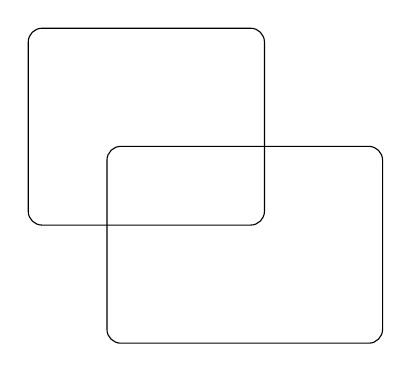
\begin{tikzpicture}[scale=1.0]
			\draw[rounded corners=5pt]  (1.0,1.0) rectangle (4.0,3.5);
			\draw[rounded corners=5pt]  (2.0,2.0) rectangle (5.5,-0.5); 
	\end{tikzpicture} }
\end{example} 
\begin{exercise}[\cancel{\faCalculator}]
	Pour chacun des couples de nombres suivants, donner la décomposition en facteurs premiers de leur plus grand commun diviseur, et de leur plus petit commun multiple.
	\begin{multicols}{3}
		\begin{enumerate}[label=\alph*),leftmargin=*]
			\item $2\times 5^2\times 7$ et $2\times 5\times 7$
			\item $2\times 5^2\times 7$ et $2\times 5\times 7^2$
			\item $2\times 3$ et $2\times 3\times 5$.
			\item $2\times 3\times 5$ et $3\times 5\times 5$
			\item $2\times 3^2\times 5$ et $3\times 5\times 5$
			\item $2\times 3^2\times 5^3$ et $3^5\times 5$
		\end{enumerate}
	\end{multicols} 
\end{exercise}
\noindent   	\parbox[position=t]{0.2\linewidth}{
	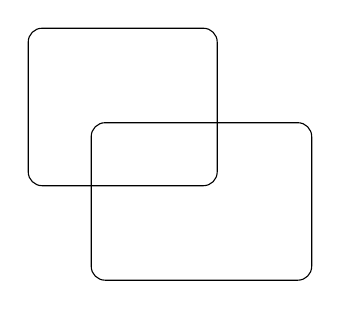
\begin{tikzpicture}[scale=0.8]
		\draw[rounded corners=5pt]  (1.0,1.0) rectangle (4.0,3.5);
		\draw[rounded corners=5pt]  (2.0,2.0) rectangle (5.5,-0.5); 
\end{tikzpicture} }\hfill 	\parbox[position=t]{0.2\linewidth}{
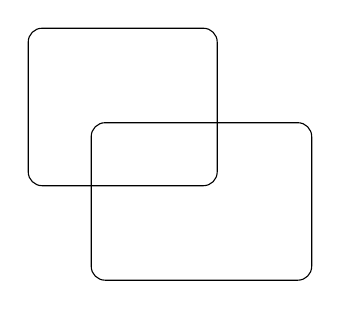
\begin{tikzpicture}[scale=0.8]
\draw[rounded corners=5pt]  (1.0,1.0) rectangle (4.0,3.5);
\draw[rounded corners=5pt]  (2.0,2.0) rectangle (5.5,-0.5); 
\end{tikzpicture} }\hfill 	\parbox[position=t]{0.2\linewidth}{
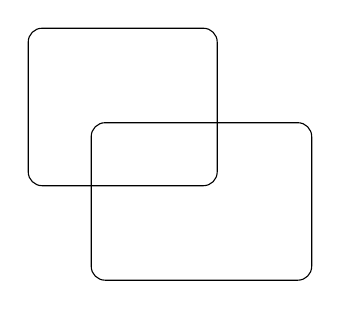
\begin{tikzpicture}[scale=0.8]
\draw[rounded corners=5pt]  (1.0,1.0) rectangle (4.0,3.5);
\draw[rounded corners=5pt]  (2.0,2.0) rectangle (5.5,-0.5); 
\end{tikzpicture} }\hfill 	\parbox[position=t]{0.2\linewidth}{
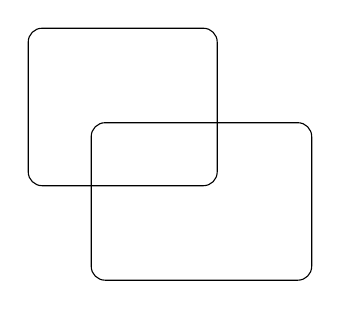
\begin{tikzpicture}[scale=0.8]
\draw[rounded corners=5pt]  (1.0,1.0) rectangle (4.0,3.5);
\draw[rounded corners=5pt]  (2.0,2.0) rectangle (5.5,-0.5); 
\end{tikzpicture} }	

\noindent \parbox[position=t]{0.2\linewidth}{
	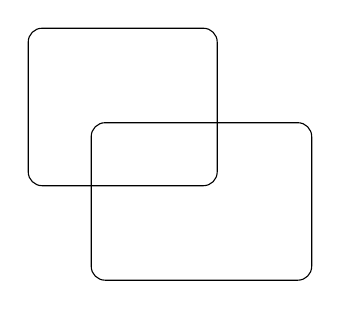
\begin{tikzpicture}[scale=0.8]
\draw[rounded corners=5pt]  (1.0,1.0) rectangle (4.0,3.5);
\draw[rounded corners=5pt]  (2.0,2.0) rectangle (5.5,-0.5); 
\end{tikzpicture} }	 \hfill \parbox[position=t]{0.2\linewidth}{
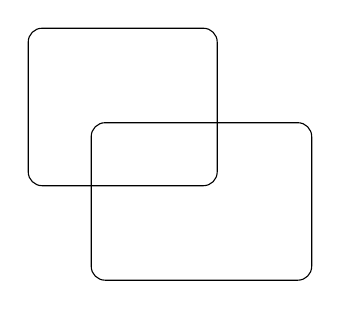
\begin{tikzpicture}[scale=0.8]
\draw[rounded corners=5pt]  (1.0,1.0) rectangle (4.0,3.5);
\draw[rounded corners=5pt]  (2.0,2.0) rectangle (5.5,-0.5); 
\end{tikzpicture} }\hfill \parbox[position=t]{0.2\linewidth}{
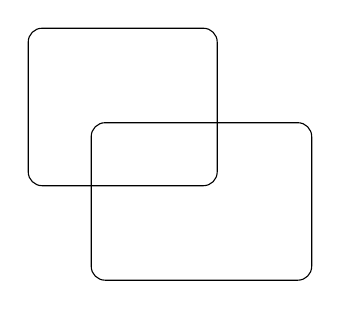
\begin{tikzpicture}[scale=0.8]
\draw[rounded corners=5pt]  (1.0,1.0) rectangle (4.0,3.5);
\draw[rounded corners=5pt]  (2.0,2.0) rectangle (5.5,-0.5); 
\end{tikzpicture} }\hfill \parbox[position=t]{0.2\linewidth}{
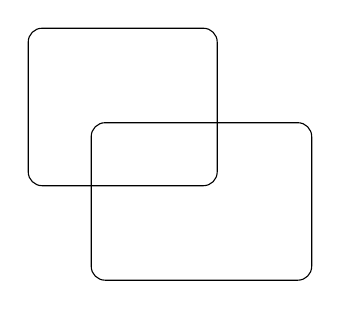
\begin{tikzpicture}[scale=0.8]
\draw[rounded corners=5pt]  (1.0,1.0) rectangle (4.0,3.5);
\draw[rounded corners=5pt]  (2.0,2.0) rectangle (5.5,-0.5); 
\end{tikzpicture} }

\begin{exercise}[\cancel{\faCalculator}]\hfill
	\begin{enumerate}[label=\alph*),leftmargin=*]
		\item $196=2^2\times 7^2$.   	Donner la décomposition en facteurs premiers de $1960$.
		\item La comète de Bailey est visible depuis la terre tous les 196 ans. Celle de Cayley est visible tous les 70 ans. Sachant que les comètes ont été vues en 1170. Quand pourra-t-on apercevoir les 2 comètes dans la même année ?
	\end{enumerate}
\end{exercise} 

\begin{exercise}[Brevet Métropole 2019]
	Le capitaine d'un navire possède un trésor constituée de $69$ diamants, \numprint{1150} perles et \numprint{4140} pièces d'or. 
	\begin{enumerate}[label=\alph*),leftmargin=*]
		\item À l'aide de la calculatrice, décomposer 69 ; \numprint{1150} et \numprint{4140} en produits de facteurs premiers.
		\item Le capitaine partage équitablement le trésor entre les marins.
		
		Combien y-a-t-il de marins sachant que toutes les pièces, perles et diamants ont été distribués ?
	\end{enumerate}
\end{exercise}
%----------------------------------------------------------------------------------------
%	 
%----------------------------------------------------------------------------------------

\newpage 
\begin{proof}[solution de l'exercice \ref{chapter02:exercice:ap02}]\hfill 
	\begin{enumerate}[label=\arabic*),leftmargin=*]
		\item  
		\begin{enumerate}[label=\alph*),leftmargin=*] 
		\item	Aire totale : $620 \times 240 + 240^2 = \numprint{206400}$~m$^2$, soit 20,64 ha ; donc on peut y faire paître au maximum : 
		$20,64 \times 12 = 247,68$, soit un maximum de 247 chèvres.  
		\item  
		Les 247 chèvres donneront en moyenne par jour : 
		$247 \times 1,8 = 444,6$~litres de lait.
	\end{enumerate} 
	\item Volume de la cuve B : $V_{\text{B}} = \pi \times  5^2 \times 7,6 = 190\pi \approx 596,9$~dm$^3$.  
	Il va donc acheter une cuve B.
\end{enumerate} 
\end{proof} 
\begin{proof}[solution de l'exercice \ref{chapter02:exercice:ap03}]\hfill  
	\begin{enumerate}
		\item $V_{\text{crème}} = 20^2 \times \pi \times = 400 \times  5 \times \pi = \numprint{2000}\pi ~\si{\milli\meter^3}$.
		
		Le volume de crème contenu dans un macaron est de $\numprint{2000}\pi$~$\left(\text{mm}^3\right)$.
		\item 1L = 1 dm$^3$ soit 100 cL = \numprint{1000000} mm$^3$ ou 1 cL = \numprint{10000}~\si{\milli\meter^3}.
		
		30 cL de crème correspondent  donc à $30 \times\numprint{10000} = \numprint{300000}~\si{\milli\meter^3}$..
		
		Je calcule : $\dfrac{\numprint{300000}}{\numprint{2000}\pi} \approx 47,7$~(macarons).
		
		Alexis peut confectionner 47 macarons.
	\end{enumerate}
\end{proof}

\begin{cBox}
	Pour obtenir la décomposition en facteurs premiers du plus petit commun multiple  :
	\begin{itemize}
		\item Je décompose les deux nombres en facteurs premiers
		\item J'établis la liste de tous les nombres premiers présents dans les deux décompositions
		\item Si un facteur premier n'apparaît qu'une fois dans une des décomposition, il garde son ordre de multiplicité.
		\item Si un facteur premier apparaît dans les deux listes, on lui attribue l'ordre de multiplicité le plus grand.
	\end{itemize}
\end{cBox}
\begin{cBox}
	Pour obtenir la décomposition en facteurs premiers du plus grand commun diviseur :
	\begin{itemize}
		\item Je décompose les deux nombres en facteurs premiers
		\item J'établis la liste de tous les nombres premiers présents dans les deux décompositions
		\item Seul un facteur premier commun aux deux décompositions sera facteurs premiers du PGCD. Sa multiplicité est la plus petite des multiplicités.
	\end{itemize}
\end{cBox}

%----------------------------------------------------------------------------------------
%	 
%----------------------------------------------------------------------------------------

\newpage 
\Tableau[Metre,  FlechesH, NbLignes=1] % FlechesH,
\Tableau[Gramme,FlechesH,  NbLignes=1] % FlechesH,
%\Tableau[Litre,FlechesH,  NbLignes=1] % FlechesH,  
\Tableau[Carre, Colonnes, FlechesH,Are, NbLignes=4] %FlechesH,Are, 
\Tableau[Cube,Colonnes,FlechesH, Capacite, NbLignes=4] %FlechesH, Capacite, 

 
%----------------------------------------------------------------------------------------
%	POSTER
%----------------------------------------------------------------------------------------
\clearpage
\loadgeometry{fullwidthlayout}  
\pagestyle{plain.scrheadings} % Print headers again  
\KOMAoptions{
	headwidth=textwithmarginpar,
	headsepline=true,
	headsepline= 0.5pt,
	footwidth=textwithmarginpar, 
}      
\doublespacing 


\tikzset{
	set angles for level/.style={level #1/.append style={sibling angle=360/(\the\tikznumberofchildren+4)}},
	level/.append code={
		\edef\tempa{#1}\edef\tempb{1}
		\ifx\tempa\tempb\tikzset{level 1/.append style={sibling angle=360/\the\tikznumberofchildren}}\else\tikzset{set angles for level=#1}\fi},
	%     set angles for level=#1},% solution 1
	non-concept/.style={
		rectangle,
		text width=15em,
		text=black,
		align=left,
		font=\large,
	},
	cncc/.style={ edge from parent path={ (\tikzparentnode.#1) to [bend right] (\tikzchildnode)   } },
}

\hvFloat*[fullpage,  capPos=after]{figure}%
{
	\begin{tikzpicture}[level 1 concept/.append style={font=\large, level distance=150} ] 
		\clip(-21,-14) rectangle (0,14.0);
		\path[mindmap, concept color=Aquamarine, grow cyclic]
		node[concept] {$a,b\in\mathbb{R}$, $b\neq0$\\ $\frac{a}{b}$}%[clockwise from=45]
		child[level distance=8cm, concept color=blue!20!white] {
			node[concept, text width=7cm, rectangle, rounded corners] (def) {Inverse de $b\neq 0$ se note $\frac{1}{b}$\\ $ b\times \frac{1}{b}=1$ }
			child[level distance=7.5cm] { node[non-concept, align=center] {Inverse de $\frac{a}{b} = \frac{1}{\frac{a}{b}}=\frac{b}{a}$} edge from parent[cncc=west] }
			child[level distance=5cm] { node[non-concept] { L'inverse de $0$ n'existe pas $\cancel{\frac{1}{0}}$} edge from parent[cncc=south west] }  
		}
		child[level distance=7cm, concept color=Pink]  { node[concept, text width=7cm, rectangle, rounded corners ] {Fraction comme multiplication :\\ $\frac{a}{b}=a\times \frac{1}{b}$} 
			[clockwise from=90]
			child[level distance=8cm] { node[non-concept] {L'unité :\\
					$\frac{b}{b}=b\times \frac{1}{b}=1$	} edge from parent[cncc= east] }
			child[level distance=5cm] { node[non-concept] {Fractions de fractions :\\
					$\frac{\frac{a}{b}}{\frac{c}{d}}=\frac{a}{b}\times \frac{1}{\frac{c}{d}}=\frac{a}{b}\times \frac{d}{c}$	} edge from parent[cncc= south] }
			child[level distance=6cm] { node[non-concept] {$\frac{a}{b}\times c =\frac{a\times c}{b} = a\times \frac{c}{b}$} edge from parent[cncc=south west] } 
		}
		child[level distance=8cm, concept color=Bisque]{ node[concept, text width=7cm, rectangle, rounded corners ] {Multiplication de fractions :\\ $\frac{a}{b}\times \frac{c}{d}=\frac{a\times c}{b\times d}$} 
			[clockwise from=45]
			%			child[level distance=5cm] { node[non-concept] {Establishing Trust \& Intimacy with the Client} edge from parent[cncc=east] }
			child[level distance=7.5cm] { node[non-concept] {Simplification/Amplification :\\ $\frac{a}{b}=\frac{a}{b}\times \frac{c}{c}= \frac{a\times c}{b\times c}$} edge from parent[cncc=  east] }    
			child[level distance=8cm] { node[non-concept] {Règles des signes :\\ $\frac{-a}{b}=-\frac{a}{b}=\frac{a}{-b}$\\ $\frac{-a}{-b}=\frac{a}{b}$} edge from parent[cncc=south   ] }    
		}
		child[level distance=7cm, concept color=AntiqueWhite]  { node[concept, text width=7cm, rectangle, rounded corners] {Fraction comme quotient :\\ $\frac{a}{b}=a\divisionsymbol b$} 
			[clockwise from=-45]
			child[level distance=7.5cm] { node[non-concept, text width=10cm  ] {Diviser revient à multiplier par l'inverse : \\ $\frac{a}{b}\divisionsymbol \frac{c}{d}=\frac{\frac{a}{b}}{\frac{c}{d}}=\frac{a}{b}\times \frac{d}{c}$} edge from parent[cncc= east] }  
		}   
		child[level distance=8cm, concept color=Cyan]  { node[concept, text width=7cm, rectangle, rounded corners] {Sommes de fractions :\\ Ramener au même dénominateur} 
			[clockwise from=0]
			%			child[level distance=5cm] { node[non-concept] {Establishing Trust \& Intimacy with the Client} edge from parent[cncc=west] }
			%			child[level distance=5cm] { node[non-concept] {Coaching Presence} edge from parent[cncc=west] } 
			child[level distance=5cm] { node[ non-concept , text width=8cm,] { $\frac{a}{b}+\frac{c}{d}=\frac{a\times d}{b\times d}+ \frac{c\times b}{d\times b}=\frac{ad+bc}{bd}$} edge from parent[cncc=north] } 
			%			child[level distance=5cm] { node[non-concept] {Coaching Presence} edge from parent[cncc=east] }     
		}; 
	\end{tikzpicture} 
}%
%[A float]%
{Règles opératoires des écritures fractionnaires}{poster:fractions}


\hvFloat*[fullpage, capPos=after]{figure}%
{
	\begin{tikzpicture}[level 1 concept/.append style={font=\large, level distance=150} ]
		\clip(0,-14.0) rectangle (21,14.0);
		\path[mindmap, concept color=Aquamarine, grow cyclic]
		node[concept] {$a,b\in\mathbb{R}$, $b\neq0$\\ $\frac{a}{b}$}%[clockwise from=45]
		child[level distance=8cm, concept color=blue!20!white] {
			node[concept, text width=7cm, rectangle, rounded corners] (def) {Inverse de $b\neq 0$ se note $\frac{1}{b}$\\ $ b\times \frac{1}{b}=1$ }
			child[level distance=7.5cm] { node[non-concept, align=center] {Inverse de $\frac{a}{b} = \frac{1}{\frac{a}{b}}=\frac{b}{a}$} edge from parent[cncc=west] }
			child[level distance=5cm] { node[non-concept] { L'inverse de $0$ n'existe pas $\cancel{\frac{1}{0}}$} edge from parent[cncc=south west] }  
		}
		child[level distance=7cm, concept color=Pink]  { node[concept, text width=7cm, rectangle, rounded corners ] {Fraction comme multiplication :\\ $\frac{a}{b}=a\times \frac{1}{b}$} 
			[clockwise from=90]
			child[level distance=8cm] { node[non-concept] {L'unité :\\
					$\frac{b}{b}=b\times \frac{1}{b}=1$	} edge from parent[cncc= east] }
			child[level distance=5cm] { node[non-concept] {Fractions de fractions :\\
					$\frac{\frac{a}{b}}{\frac{c}{d}}=\frac{a}{b}\times \frac{1}{\frac{c}{d}}=\frac{a}{b}\times \frac{d}{c}$	} edge from parent[cncc= south] }
			child[level distance=6cm] { node[non-concept] {$\frac{a}{b}\times c =\frac{a\times c}{b} = a\times \frac{c}{b}$} edge from parent[cncc=south west] } 
		}
		child[level distance=8cm, concept color=Bisque]{ node[concept, text width=7cm, rectangle, rounded corners ] {Multiplication de fractions :\\ $\frac{a}{b}\times \frac{c}{d}=\frac{a\times c}{b\times d}$} 
			[clockwise from=45]
			%			child[level distance=5cm] { node[non-concept] {Establishing Trust \& Intimacy with the Client} edge from parent[cncc=east] }
			child[level distance=7.5cm] { node[non-concept] {Simplification/Amplification :\\ $\frac{a}{b}=\frac{a}{b}\times \frac{c}{c}= \frac{a\times c}{b\times c}$} edge from parent[cncc=  east] }    
			child[level distance=8cm] { node[non-concept] {Règles des signes :\\ $\frac{-a}{b}=-\frac{a}{b}=\frac{a}{-b}$\\ $\frac{-a}{-b}=\frac{a}{b}$} edge from parent[cncc=south   ] }    
		}
		child[level distance=7cm, concept color=AntiqueWhite]  { node[concept, text width=7cm, rectangle, rounded corners] {Fraction comme quotient :\\ $\frac{a}{b}=a\divisionsymbol b$} 
			[clockwise from=-45]
			child[level distance=7.5cm] { node[non-concept, text width=10cm  ] {Diviser revient à multiplier par l'inverse : \\ $\frac{a}{b}\divisionsymbol \frac{c}{d}=\frac{\frac{a}{b}}{\frac{c}{d}}=\frac{a}{b}\times \frac{d}{c}$} edge from parent[cncc= east] }  
		}   
		child[level distance=8cm, concept color=Cyan]  { node[concept, text width=7cm, rectangle, rounded corners] {Sommes de fractions :\\ Ramener au même dénominateur} 
			[clockwise from=0]
			%			child[level distance=5cm] { node[non-concept] {Establishing Trust \& Intimacy with the Client} edge from parent[cncc=west] }
			%			child[level distance=5cm] { node[non-concept] {Coaching Presence} edge from parent[cncc=west] } 
			child[level distance=5cm] { node[ non-concept , text width=8cm,] { $\frac{a}{b}+\frac{c}{d}=\frac{a\times d}{b\times d}+ \frac{c\times b}{d\times b}=\frac{ad+bc}{bd}$} edge from parent[cncc=north] } 
			%			child[level distance=5cm] { node[non-concept] {Coaching Presence} edge from parent[cncc=east] }     
		}; 
	\end{tikzpicture}
}%
%[A float]%
{Partie 2}{}

\clearpage
%----------------------------------------------------------------------------------------
%	 
%----------------------------------------------------------------------------------------
\cleardoublepage
\end{document}
 